\section{Data Processing: Basic Concepts and External Sorting}

\paragraph{Different Cost Models for Algorithms}
\begin{itemize}
\item \textbf{RAM model}
  \begin{itemize}
  \item Every basic operation takes constant time
  \item Memory access, simple additions, does not matter
  \end{itemize}

\item \textbf{I/O model}
  \begin{itemize}
  \item Transfer data from disk in large blocks / pages
  \item Count number of I/Os performed
  \item \textbf{Assumption:} I/Os dominate total cost, any
    I/O as good as another one $\rightarrow$ not always true
  \end{itemize}

\item \textbf{More sophisticated cost models}
  \begin{itemize}
  \item Create cost function which mixes CPU, memory
    access, I/O costs
  \item Differentiate types of access patterns
    (sequential, random, semi-random, etc)
  \item Complexity can grow very high, very quickly
  \end{itemize}
\end{itemize}

\paragraph{Example for first external memory algorithm: Sorting}

\textbf{Why sorting?}
\begin{itemize}
\item Important in data processing (relational queries)
\item Used for eliminating duplicates (SELECT DISTINCT)
\item Bulk loading B+ trees (need to first sort leaf level pages)
\item Data requested in sorted order
\item Some join algorithms use sorting
\item Some MapReduce implementations use sorting to group keys
  for reducers
\end{itemize}

\paragraph{Example: Sorting}
If we want to sort 1 TB of data with 1 GB of RAM we
cannot rely on normal in-memory sorting implementation
using for example QuickSort.

\textbf{Idea:} 2-Way External Merge Sort


\paragraph{2-Way External Merge Sort: Phase 1}
\begin{itemize}
\item Based on merge sort (now with two phases)
\item Read one page at a time from disk
\item Sort it in memory (e.g. QuickSort)
\item Write it to disk as one temporary file (called ``run'')
  \begin{itemize}
  \item Given an input with N pages, Phase 1 produces N runs
  \end{itemize}
\item Only one buffer page used
\end{itemize}

\begin{figure}[h]
  \begin{minipage}{1.0\linewidth}
    \begin{center}
      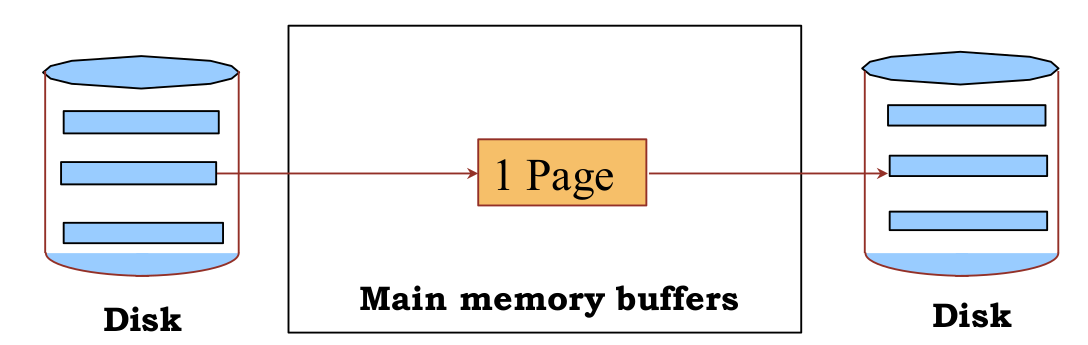
\includegraphics[scale=0.17]{graphics/external-msort-v1}
    \end{center}
  \end{minipage}
\end{figure}

\paragraph{Phase 1: Example}
\begin{figure}[h]
  \begin{minipage}{1.0\linewidth}
    \begin{center}
      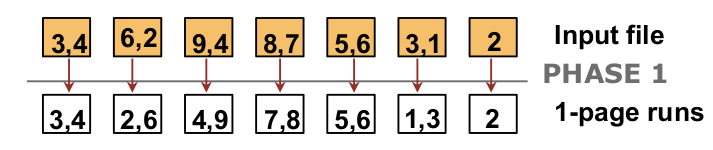
\includegraphics[scale=0.2]{graphics/phase1-ex}
    \end{center}
  \end{minipage}
\end{figure}
\begin{itemize}
\item Assuming the input file has N data pages of size M
\item The cost of Phase 1 is:
  \begin{itemize}
  \item in terms of number or I/Os: 2N
  \item in terms of computational steps: $\mathcal{O}(N M \log(M))$
  \end{itemize}
\end{itemize}


\paragraph{2-Way External Merge Sort: Phase 2}
Make multiple passes to merge runs
\begin{itemize}
\item Pass 1: Merge two runs of length 1 (page)
\item Pass 2: Merge two runs of length 2 (pages)
\item ... until 1 run of length N
\item Three buffer pages used
\end{itemize}

\begin{figure}[h]
  \begin{minipage}{1.0\linewidth}
    \begin{center}
      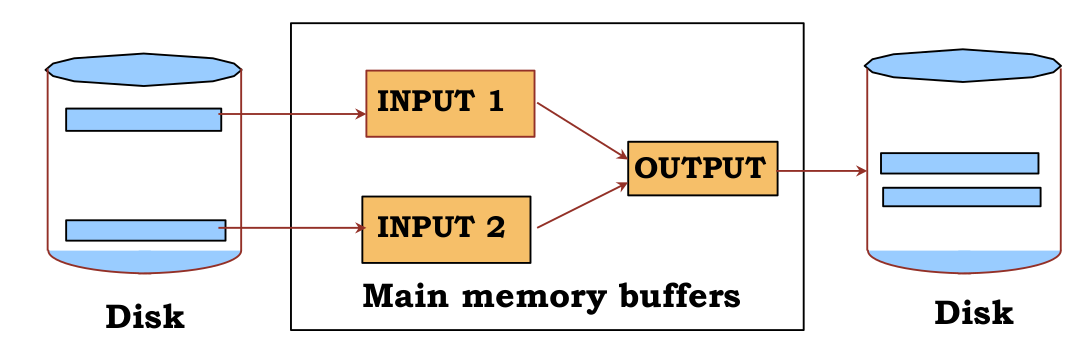
\includegraphics[scale=0.18]{graphics/phase2}
    \end{center}
  \end{minipage}
\end{figure}



\paragraph{2-Way External Merge Sort: Example}

\begin{figure}[h]
  \begin{minipage}{1.0\linewidth}
    \begin{center}
      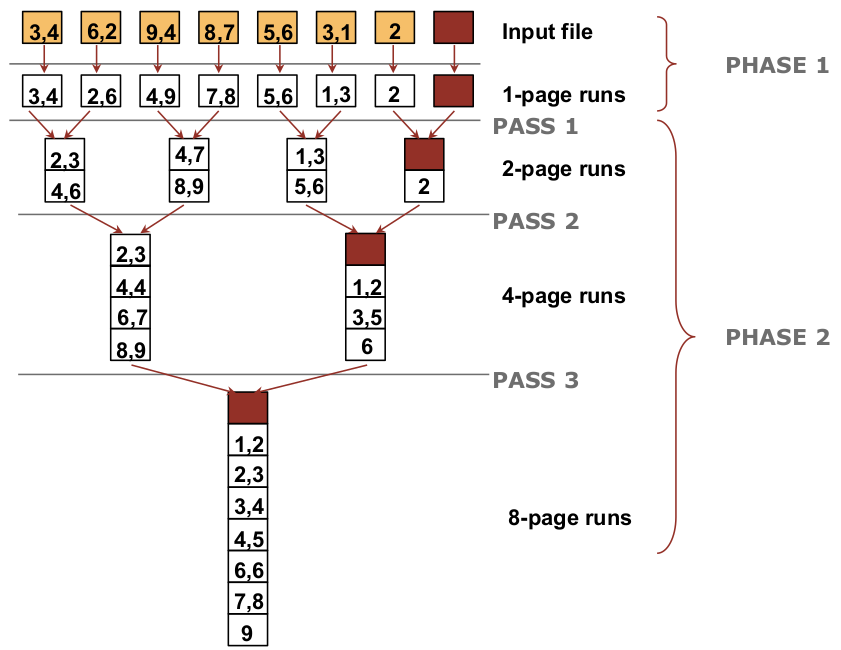
\includegraphics[scale=0.18]{graphics/phase2-ex}
    \end{center}
  \end{minipage}
\end{figure}



\paragraph{2-Way External Merge Sort: Analysis}
\begin{itemize}
\item Total I/O cost for sorting file with N pages
\item Cost of Phase 1 = 2 N
\item Number of passes in Phase 2 = $\lceil \log_2 N \rceil$
\item Cost of each pass in Phase 2 = 2 N
\item Cost of Phase 2 = $2 N \cdot \lceil \log_2 N \rceil$
\item Total cost = $2N (\lceil \log_2 N \rceil + 1)$
\end{itemize}



\paragraph{Can we do better?}
\begin{itemize}
\item The cost depends on the \#passes
\item \#passes depends on
  \begin{itemize}
  \item fan-in during the merge phase
  \item the number of runs produced by phase 1
  \end{itemize}
\end{itemize}



\paragraph{Multi-Way External Merge Sort}
\begin{itemize}
\item Phase 1: Read B pages at a time, sort B pages in main
  memory, and write out B pages
\item \textbf{Length of each run = B pages}
\item Assuming N input pages, number of runs = N/B
\item Cost of Phase 1 = 2N
\end{itemize}

\begin{figure}[h]
  \begin{minipage}{1.0\linewidth}
    \begin{center}
      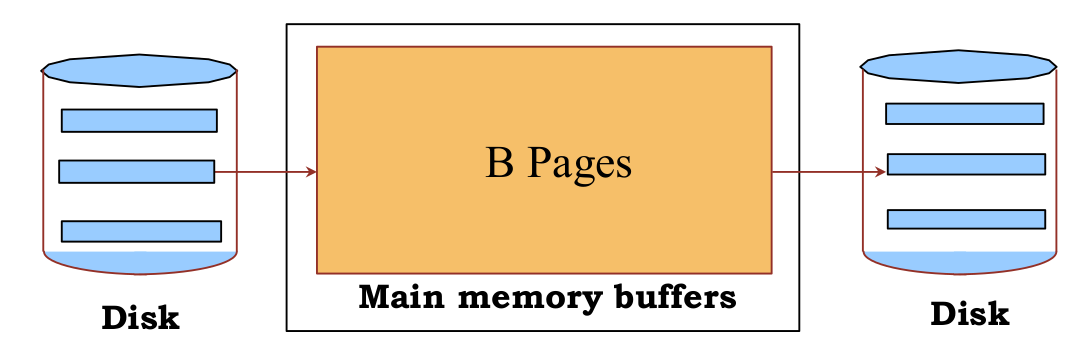
\includegraphics[scale=0.17]{graphics/multi-way-external-merge-sort}
    \end{center}
  \end{minipage}
\end{figure}



\paragraph{2-Way External Merge Sort: Example}
Number of buffer pages B = 4

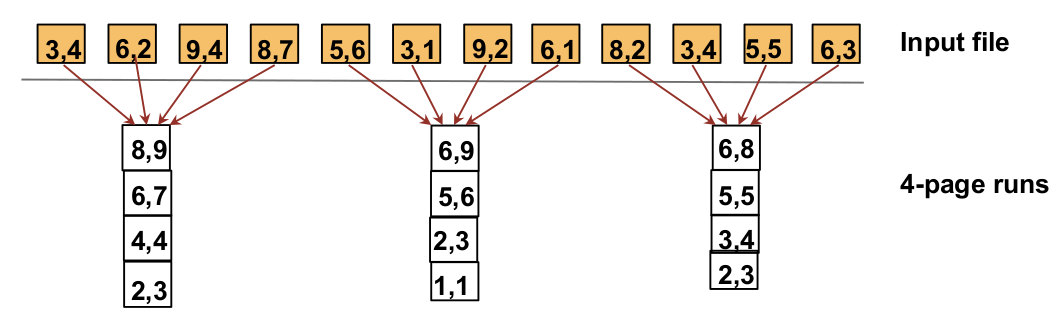
\includegraphics[scale=0.18]{graphics/B=4}

\paragraph{Multi-Way External Merge Sort Phase 2}
\begin{itemize}
\item Phase 2: Make multiple passes to merge runs
  \begin{itemize}
  \item Pass 1: Produce runs of length $B(B-1)$ pages
  \item Pass 2: Produce runs of length $B(B-1)^2$ pages

    $\vdots$

  \item Pass P: Produce runs of Length $B(B-1)^P$ pages
  \end{itemize}
\end{itemize}

\paragraph{Multi-Way External Merge Sort: Analysis}
Total I/O cost for sorting file with N pages

\begin{itemize}
\item Cost of Phase 1 = $2N$
\item If number of passes in Phase 2 is P then: $B(B-1)^P = N$
\item P = $\lceil \log_{B-1}\lceil N/B \rceil\rceil$
\item Cost of each pass = $2N$
\item Cost of Phase 2 =
  $2N \cdot \lceil \log_{B-1} \lceil N / B\rceil \rceil$
\item Total cost =
    $2N \cdot (\lceil \log_{B-1} \lceil N / B\rceil \rceil + 1)$
\item compared to $2N (\lceil \log_2 N \rceil + 1)$
\end{itemize}

\paragraph{Can we produce runs larger than the RAM size?}

\textbf{Tournament sort (a.k.a ``heapsort'',
  ``replacement selection sort'')}
\begin{itemize}
\item use 1 buffer page as the input buffer and 1 buffer page as
  the output buffer
\item Maintain 2 Heap structures in the remaining B-2 pages
  (H1, H2)
\item Read B-2 pages of records and insert them into H1
\item While there are still records left
  \begin{itemize}
  \item get the ``min'' record m from H1 and send it to the output
    buffer
  \item If H1 is empty then start a new run and put all the records
    in H2 to H1
  \item read another record r from the input buffer
  \item if r < m then put it in H2, otherwise put it in H1
  \end{itemize}
\item Finish the current run by outputting all the records in H1
\item If there is something left in H2, output them as a new run
\end{itemize}

\paragraph{More on Heapsort}
\begin{itemize}
\item Fact: average length of a run in heapsort is 2(B-2)
  \begin{itemize}
  \item B-2 pages are used for the heaps
  \item (B-2) + 1/2 (B-2) + 1/4 (B-2) + 1/8 (B-2) + $\ldots$
    $\approx$ 2(B-2)
  \end{itemize}
\item Worst-Case:
  \begin{itemize}
  \item min length of a run is
  \item this arises if all elements are smaller than elements in H1
  \end{itemize}
\item Best-Case:
  \begin{itemize}
  \item max length of a run is entire size of input
  \item this arises if all elements are already sorted (close to sorted)
  \end{itemize}
\item QuickSort is faster, but longer and fewer runs often mean
  fewer passes!
\end{itemize}

\paragraph{External Merge Sort: Possible Optimizations}
\begin{itemize}
\item In Phase 2 read/write blocks of pages instead of single page
\item Double buffering: to reduce I/O wait time, \textit{prefetch}
  into ``shadow block''
\end{itemize}

\paragraph{Key Points (External Sorting)}
\begin{itemize}
\item When data is much too big to fit in memory our
  ``normal'' best algorithms might not be the best
\item External sorting
  \begin{itemize}
  \item sorting with two (or more) disks
  \item use merge sort (2-phase)
  \end{itemize}
\item Optimizations
  \begin{itemize}
  \item Utilize memory to the fullest
  \item use heap/replacement sort to reduce \#runs
  \item Read sequences of pages from disk
  \item keep disks ``busy''
  \end{itemize}
\end{itemize}
% LocalWords:  MapReduce QuickSort heapsort prefetch
